\documentclass[UTF8,a4paper,11pt]{ctexart}

\usepackage{geometry}
\geometry{left=2.5cm,right=2.5cm,top=2.5cm,bottom=2.5cm}
\usepackage{booktabs}
\usepackage{array}
\usepackage{enumitem}
\usepackage{xcolor}
\usepackage{listings}
\usepackage{hyperref}
\usepackage{caption}
\usepackage{longtable}
\usepackage{float}
\floatplacement{table}{H}
\floatplacement{figure}{H}
\usepackage{graphicx}
\usepackage{subcaption}
\graphicspath{{figures/}}
\usepackage{tikz}
\usetikzlibrary{arrows.meta,positioning,shapes.geometric}

\hypersetup{colorlinks=true,linkcolor=black,urlcolor=blue!50!black}
\lstset{
  basicstyle=\ttfamily\small,
  breaklines=true,
  frame=single,
  rulecolor=\color{gray!40},
  backgroundcolor=\color{gray!6},
  columns=fullflexible,
  keepspaces=true,
  showstringspaces=false
}
\captionsetup{font=small,labelfont=bf}

\title{\textbf{Material Magician：东方醒狮数字展厅}\\[4pt]
\large 从一尊 AI 素模到可漫游、可赋材、可共创的三维叙事空间}
\author{课程项目报告}
\date{2026 年 11 月}

\begin{document}

\maketitle

\begin{abstract}
本项目以中国传统南狮为题材，构建了一个基于 Web 的三维互动展厅。主角是一尊由 AI 生成的 Q 版「小狮童」素模（约 19.7 万三角面）；项目在同一副骨架上实现了九套材质、九段真实骨骼动作、三套布景光调、五处部位热点、五章舞狮故事与四章练功内容，并提供第三人称角色漫游与门外街市。生成式能力来自 Aholo Lux3D（文生 3D、材质迁移）与 SpatialGen（三维场景生成，输出 3DGS）。本文介绍系统的设计动机、总体架构、各子系统的关键实现与参数选择，说明资产构成与加载预算，总结开发过程中遇到的问题与解决方式，并对当前能力边界与后续工作给出判断。

\vspace{6pt}
\noindent\textbf{关键词：}数字展陈；Three.js；PBR 材质；骨骼动画；3DGS；生成式三维
\end{abstract}

\tableofcontents
\newpage

% ============================================================
\section{引言}

\subsection{背景}
舞狮是中国南方极具代表性的民俗表演。一头南狮的完整生命周期包括扎作、开光、起势、采青、收势，台下还有马步、石锁、走桩、鼓点等长期训练。传统展陈通常以实物、照片或视频呈现，观众看到的是「结果」，很难理解三件事：狮头是怎么被扎出来的、动作是怎么被训练出来的、材质如何改变同一形体的观感。

数字展陈提供了另一种可能：把一尊角色做成可旋转、可换材、可播放动作、可进入空间的数字对象，让「形—材—事」三层同时可见。但这也带来工程上的矛盾——高精度模型体积大、材质变体多、动作文件重，而网页的首屏预算有限。

\subsection{问题定义}
项目要回答的不是「如何做一个好看的模型页」，而是：
\begin{enumerate}[itemsep=2pt]
  \item 如何在浏览器里承载一尊约 20 万面的角色，并支持多套材质与多段骨骼动作的自由组合；
  \item 如何让生成式三维能力（文生 3D、材质迁移、场景生成）真正进入展陈流程，而不是停留在参数演示；
  \item 如何用 3D 讲清楚一个文化对象——不只是展示，而是解释。
\end{enumerate}

\subsection{目标}
\begin{itemize}[itemsep=2pt]
  \item 在单页内完成「看形—换材—播动作—读故事—走进空间」的闭环；
  \item 首屏可用：只加载当前材质，其余按需；装饰资产延迟加载；
  \item 每个生成资产都能追溯到具体的 API 与任务 ID，形成可复现的管线。
\end{itemize}

\subsection{主要工作与贡献}
\begin{enumerate}[itemsep=2pt]
  \item \textbf{材质与动作解耦}：九套材质可播放任意一段动作，切换材质不打断动作；
  \item \textbf{程序化展厅}：38$\times$42$\times$10 的东方展厅，含侧室、壁龛、屏风、盘龙、宫灯与街市；
  \item \textbf{三层叙事}：部位热点（形）、材质档案（材）、故事与练功（事）；
  \item \textbf{双模漫游}：第一人称探索与第三人称角色漫游，带碰撞；
  \item \textbf{生成管线}：接入 Lux3D 文生 3D、材质迁移与 SpatialGen 3DGS 场景。
\end{enumerate}

\subsection{报告结构}
第 2 节介绍技术选型与相关工作；第 3 节给出系统架构与状态管理；第 4 节逐个说明关键实现；第 5 节统计资产与加载预算；第 6 节讨论性能取舍；第 7 节给出评测、失败案例与限制；第 8 节讨论与游戏引擎结合的可能性；第 9 节展望未来工作。

% ============================================================
\section{技术选型与相关工作}

\subsection{Web 三维}
渲染使用 Three.js 0.180，构建工具为 Vite。选择 Web 而非 Unity/Unreal 的原因有三：
\begin{itemize}[itemsep=2pt]
  \item \textbf{分享成本低}：一个链接即可打开，评审与展示不需要安装；
  \item \textbf{迭代快}：改一行代码即可热更新，适合在十几轮迭代中反复调整；
  \item \textbf{与文档同构}：HTML/CSS 天然适合做展签、面板与排版。
\end{itemize}
代价是渲染质量、资产压缩工具链与动画系统都不如原生引擎——这一点在第 8 节展开。

\subsection{资产格式}
所有角色与道具均为 GLB（glTF 二进制），PBR 材质内嵌贴图；骨骼动作来自 Mixamo，导出为独立 GLB。3DGS 场景使用压缩后的 \texttt{.spz}。选择 GLB 的原因是它是 Web 与 DCC 工具之间的事实标准：Blender、Unity、Three.js 都能直接读取。

\subsection{骨骼动画}
九段动作均为 Mixamo 骨骼（其中跳跃、滑铲、蹲伏由多段片段合并）（52 或 22 关节），每段包含完整角色网格、蒙皮与动画通道。这种「一段动作带一份角色」的导出方式在网页端代价很高，但好处是零配置即可播放——不需要运行时重定向。

\subsection{生成式三维}
\begin{itemize}[itemsep=2pt]
  \item \textbf{Lux3D}：文生 3D（\texttt{text-to-3d}）、材质迁移（\texttt{material-transfer}）、多格式导出、部件拆分、骨骼重定向等；
  \item \textbf{SpatialGen}：通过 Aholo OpenAPI 的 \texttt{World} 接口提交场景生成，输出 3DGS（\texttt{.ply} / \texttt{.spz}）。
\end{itemize}
两者共用一套 OpenAPI 鉴权（\texttt{Authorization: <API Key>}），资产上传则走独立的 OUS 接口（\texttt{ous-token-v2}）。

% ============================================================
\section{系统架构}

\subsection{模块职责}
\begin{table}[H]
\centering
\small
\caption{主要模块}
\begin{tabular}{@{}p{2.4cm}p{5.0cm}p{6.9cm}@{}}
\toprule
模块 & 文件 & 职责 \\
\midrule
主流程 & \texttt{src/main.js} & 初始化、模式切换、交互编排、快捷键、点击拾取 \\
配置 & \texttt{src/config.js} & 材质、动作、布景、机位、视图模式、展示参数 \\
场景 & \texttt{src/scene.js} & 渲染器、灯光、三套光调、性能分级 \\
模型 & \texttt{src/model-manager.js} & 加载、归一化、LRU 缓存、材质保护 \\
动作 & \texttt{src/action-theater.js} & 骨骼动画、根位移原地化、材质借用 \\
相机 & \texttt{src/camera-controls.js} & 轨道、机位补间、第一人称、碰撞 \\
漫游 & \texttt{src/roam.js} & 第三人称移动、跑跳切换、相机跟随 \\
热点 & \texttt{src/hotspot-tour.js} & 部位热点投影、聚焦、说明卡 \\
街景 & \texttt{src/splat-street.js} & 3DGS 查看器与开关 \\
展厅 & \texttt{src/environment/} & 程序化展厅、街市、摆件、故事长廊 \\
\bottomrule
\end{tabular}
\end{table}

\subsection{总体结构}
\begin{figure}[H]
\centering
\begin{tikzpicture}[
  box/.style={draw, rounded corners=2pt, align=center, font=\footnotesize, minimum height=10mm, text width=3.2cm, fill=gray!4},
  arr/.style={-{Latex[length=2mm]}, thick, gray!60}
]
\node[box] (ui) at (0, 0) {UI 层\\面板 / 热点 / 说明卡};
\node[box] (main) at (0, -1.7) {main.js\\状态机与交互编排};
\node[box] (mm) at (-4.3, -3.6) {ModelManager\\材质加载与缓存};
\node[box] (at) at (0, -3.6) {ActionTheater\\骨骼动作与材质借用};
\node[box] (roam) at (4.3, -3.6) {RoamController\\第三人称漫游};
\node[box] (cam) at (-4.3, -5.5) {ViewerController\\轨道 / 机位 / 碰撞};
\node[box] (env) at (0, -5.5) {环境层\\展厅 / 街市 / 3DGS};
\node[box] (scene) at (4.3, -5.5) {SceneContext\\渲染器 / 灯光 / 光调};
\draw[arr] (ui) -- (main);
\draw[arr] (main) -- (mm);
\draw[arr] (main) -- (at);
\draw[arr] (main) -- (roam);
\draw[arr] (mm) -- (env);
\draw[arr] (at) -- (env);
\draw[arr] (roam) -- (env);
\draw[arr] (cam) -- (env);
\draw[arr] (scene) -- (env);
\end{tikzpicture}
\caption{系统模块关系。UI 只负责展示与事件，状态集中在 main.js，渲染与资产各自独立。}
\end{figure}

\subsection{运行流程}
\begin{lstlisting}
init:
  buildEnvironment()            // 程序化展厅 + 街市 + 摆件（异步加载）
  ModelManager.show('original') // 首屏只加载素模
  idle -> preload next material // 空闲时预取下一套

frame:
  modelManager.update(dt)       // 自动旋转、呼吸
  actionTheater.update(dt)      // 动画混合器
  roamController.update(dt)     // 漫游移动与相机跟随
  viewerControls.update(dt)     // 轨道或第一人称
  hotspotTour.update()          // 热点投影
  environment.update(t, dt)     // 盘龙、尘埃、行人
  renderer.render()
\end{lstlisting}

\subsection{状态管理}
系统有三类互斥状态：

\begin{table}[H]
\centering
\small
\caption{三种观察状态}
\begin{tabular}{@{}llll@{}}
\toprule
状态 & 相机 & 控制 & 冲突处理 \\
\midrule
展台观察 & OrbitControls & 拖动 / 滚轮 & 默认 \\
第一人称 & 自由视角 & WASD + 指针锁定 & 关闭轨道 \\
角色漫游 & 第三人称跟随 & W/S 前后、A/D 转身 & 轨道挂起 \\
\bottomrule
\end{tabular}
\end{table}

漫游期间通过 \texttt{ViewerController.setSuspended(true)} 挂起轨道控制，其 \texttt{update()} 直接返回，避免两套相机逻辑互相覆盖。退出漫游时恢复轨道并复位相机。

% ============================================================
\section{关键实现}

\subsection{材质系统}

\subsubsection{九套材质}
九套材质共享同一副几何（约 197{,}135 三角面、170{,}884 顶点），每套是独立的 GLB 文件（12--16MB），内嵌 PBR 贴图。

\begin{table}[H]
\centering
\small
\caption{九套材质与推荐光调}
\begin{tabular}{@{}clll@{}}
\toprule
编号 & 名称 & 关键参数 & 推荐光调 \\
\midrule
01 & 原始素模 & metal 0.02 / rough 0.92 & 月白·影棚 \\
02 & 鎏金 & metal 0.95 / rough 0.28 & 墨夜·聚光 \\
03 & 彩釉 & metal 0.05 / rough 0.22 & 朱砂·堂会 \\
04 & 大理石 & metal 0.02 / rough 0.45 & 月白·影棚 \\
05 & 澄明玻璃 & rough 0.05 / transmission 0.92 & 墨夜·聚光 \\
06 & 彩璃 & rough 0.12 / transmission 0.6 & 朱砂·堂会 \\
07 & 白瓷 & rough 0.15 & 月白·影棚 \\
08 & 羊毛毡 & rough 0.98 & 朱砂·堂会 \\
09 & AI 鎏金 & 迁移生成 & 墨夜·聚光 \\
\bottomrule
\end{tabular}
\end{table}

\subsubsection{加载与缓存}
首屏只加载当前材质（默认素模），其余按需。缓存上限为 2 套，超出后按最近使用时间淘汰。正在被动作模型借用的材质会被标记为 \texttt{protectedKey}，不参与淘汰——否则贴图会被释放，动作模型变黑。

\subsubsection{切换与淡入淡出}
材质切换时，旧模型透明度从 1 降到 0、新模型从 0 升到 1，时长约 520ms。若动作正在播放，则跳过淡入淡出（避免两个同位置模型叠加），改为即时替换动作网格上的材质。

\subsubsection{环境反射}
不同材质的 \texttt{envMapIntensity} 不同：金属 1.45、玻璃 1.15、彩釉/彩璃/白瓷 1.0、大理石 0.8、毛毡 0.55。这一项直接决定材质"像不像"。

\subsection{动作系统}

\subsubsection{九段动作}
\begin{table}[H]
\centering
\small
\caption{动作片段（9 段）}
\begin{tabular}{@{}llrrl@{}}
\toprule
动作 & 文件 & 时长 & 骨骼 & 播放 \\
\midrule
点头 & 点头同意.glb & 2.50s & 22 关节 & 单次 \\
跳舞 & 跳舞.glb & 1.00s & 22 关节 & 循环 \\
直拳 & 直拳.glb & 1.00s & 22 关节 & 单次 \\
翻滚 & 翻滚.glb & 1.47s & 22 关节 & 单次 \\
走路 & 走路.glb & 1.33s & 52 关节 & 循环 \\
奔跑 & 奔跑.glb & 0.93s & 52 关节 & 循环 \\
跳跃（起跳+滞空+落地） & jump-group.glb & 5.14s & 52 关节 & 单次 \\
滑铲（启动+滑行+结束） & slide.glb & 3.37s & 22 关节 & 单次 \\
蹲伏行走 & crouch-walk.glb & 2.00s & 22 关节 & 循环 \\
\bottomrule
\end{tabular}
\end{table}

\subsubsection{材质借用}
播放动作时，材质模型被隐藏，动作模型显示。若直接播放，观众看到的是动作文件自带的素模表面。因此每帧开始前，把当前材质模型的 material 克隆到动作网格：

\begin{lstlisting}
applyMaterialFrom(group) {
  const sources = collectMaterials(group);   // 当前材质
  this.releaseAppliedMaterials();            // 释放上一批克隆
  targets.forEach((mesh, i) => {
    const clone = sources[i % sources.length].clone();
    clone.transparent = false;
    clone.depthWrite = true;
    mesh.material = clone;
  });
}
\end{lstlisting}

只克隆 material、共享贴图，避免重复占显存。克隆前先把动作模型隐藏，替换完成后再显示，防止第一帧闪回素模。

\subsubsection{根位移原地化}
翻滚与奔跑的原始动画带根骨骼位移（Hips 前后 0.37--0.40）。角色被归一化到 3.25 单位高后，这段位移会把角色带出展台。处理方式是在加载时锁定根骨骼的 X、Z：

\begin{lstlisting}
const isRootBone = (n) => /(^|[.:_])(Hips|Root)$/.test(n);
// 注意：GLTFLoader 会把 "mixamorig:Hips" 洗成 "mixamorig_Hips"
for (const track of clip.tracks) {
  if (!track.name.endsWith('.position')) continue;
  if (!isRootBone(track.name.slice(0, -9))) continue;
  const v = track.values, x0 = v[0], z0 = v[2];
  for (let i = 0; i < v.length; i += 3) { v[i] = x0; v[i + 2] = z0; }
}
\end{lstlisting}

保留 Y 轴起伏，因此下蹲、腾空、翻转的高度仍然是真实的。走路原本位移仅 0.09，处理后基本无感。

\subsection{布景光调}
三套光调只改灯光、雾、背景与曝光，不重新加载模型：

\begin{table}[H]
\centering
\small
\caption{三套布景光调}
\begin{tabular}{@{}llll@{}}
\toprule
光调 & 背景 & 主光 & 适用 \\
\midrule
墨夜·聚光 & 深红暗场 & 暖金顶光 & 鎏金、默认 \\
月白·影棚 & 中性冷灰 & 冷白柔光 & 素模、白瓷 \\
朱砂·堂会 & 暗红 & 朱红侧逆光 & 彩釉、彩璃 \\
\bottomrule
\end{tabular}
\end{table}

切换时光调同步写入 \texttt{body[data-mood]}，页面四周的压暗层一起变化，避免「灯变冷了、氛围层还是暖红」的割裂。三套光调的半球光与环境光强度都经过一次整体提亮（1.25$\rightarrow$1.8、0.42$\rightarrow$0.68），以解决早期墙面过暗的问题。

\subsection{相机与观察}

\subsubsection{机位预设}
全景、狮首、侧身三个机位，使用与「复位视角」同一套补间。用户一旦拖动，立即交还 OrbitControls 并取消机位高亮。狮首机位目标点设在 y=2.9，正对狮头。

\subsubsection{视角范围}
为了让近景机位不被弹回，\texttt{minDistance} 从 4.2 放宽到 1.8，\texttt{maxDistance} 从 14 放宽到 22（配合放大后的展厅）。

\subsection{叙事内容}

\subsubsection{部位热点}
五处热点：祥云纹、卷曲鬃毛、盘扣、衣褶、布鞋。坐标不是手工摆的，而是从 GLB 顶点算出来的：

\begin{enumerate}[itemsep=2pt]
  \item 读取 POSITION，得到包围盒；
  \item 按页面规则归一化：缩放 $s = 3.25 / h$，X/Z 居中，脚底 y=0；
  \item 在目标高度区间筛顶点，取 $z$ 最大（最靠前）的点；
  \item 沿法线方向外扩约 0.1，避免标记陷进表面。
\end{enumerate}

标记是 HTML 按钮，每帧把 3D 锚点投影到屏幕坐标后定位，因此文字始终正对观众。根据「点相对模型中心是否朝向相机」做背面剔除。

\subsubsection{故事长廊}
五章：点睛、起势、采青、醉狮、收势。沿左墙排开五座石台，每座配一个符号化道具与一块墙面说明牌（Canvas 文字）。右侧面板与 3D 展台共用同一份数据（\texttt{story.js}）。

\subsubsection{练功房}
四章：扎马步、石锁、走桩、鼓点。器械放在右侧展室里。这一组补上了「台下」的叙事，与故事长廊的「台上」形成对照。

\subsection{角色漫游}
角色相对控制：\texttt{W/S} 沿朝向前后、\texttt{A/D} 原地转身、\texttt{Shift} 奔跑、\texttt{Space} 跳跃。速度做阻尼（$1-e^{-9\Delta t}$），避免起步与收步生硬；相机以 9 的平滑系数跟随在身后 7.2 单位、高 4.0。

移动时按方向转身，停下时结束动画、显示当前材质的静态模型。碰撞半径 0.62，圆形与矩形碰撞体分别覆盖柱子/摆件与墙体。

\subsection{空间与街市}

\subsubsection{展厅}
38$\times$42$\times$10，柱列 8 根，后墙有月亮门与壁龛，两侧展室通过带门洞的隔墙隔出。展厅内还有盘龙（半径 8.6 缓慢盘旋）、宫灯一对、鼓、香炉与四片屏风（后减为一片）。

\subsubsection{街市}
右墙开门（3.2 宽、3.9 高），红毯从展台铺到门口，门上有「街市」匾额与门灯。门外是一条东西向小街：夯土路面、两排木构店铺、街尾城门、街灯与三个独立行人（沿街往返、带步幅起伏与摆臂）。

\subsection{3DGS 街景：一次失败的接入}

通过 \texttt{POST /world/v1/generations} 提交文本提示词，约 16 分钟生成，输出 \texttt{.ply}（32.4MB）与压缩 \texttt{.spz}（7.9MB）。前端最初使用 \texttt{@mkkellogg/gaussian-splats-3d} 0.4.7 的独立 Viewer 渲染。

实测发现两个问题：
\begin{enumerate}[itemsep=2pt]
  \item \texttt{.spz} 是 v3 格式，而该库只解析到 v2，直接报 \\texttt{deserializePackedGaussians: version not supported: 3}；
  \item 换用 \texttt{.ply} 后可以加载（约 10--14 秒），但在纯 CPU 环境下画面全黑，无法确认是取景还是软件渲染限制。
\end{enumerate}

因此当前版本把入口改为同一空间的全景图（\texttt{panoUrl}，1.1MB，等距柱状）：\\texttt{PanoStreet} 用球面贴图 + 拖拽环视 + 滚轮缩放，秒开，且在任何设备上都有画面。3DGS 文件与查看器代码仍保留在仓库，作为后续升级的接口。

\subsection{街市与传送门}

展厅右侧开门通向一条长安街市，可从侧栏「PORTAL」一键传送，也可以沿红毯步行出门。

街市由三类内容组成：
\begin{itemize}[itemsep=2pt]
  \item \textbf{生成式建筑}：酒楼 6 件（\texttt{street-inn}，9.5 高，两侧各三间）、阁楼（\texttt{street-pavilion}，10 高）、门楼（\texttt{street-gate}，12 高）；
  \item \textbf{摊位与道具}：五处木台摊位，桌面上摆酒坛、生菜、醒狮鼓、香炉、宫灯，均为 Lux3D 生成资产；
  \item \textbf{NPC}：三个独立行人，沿街往返并带摆臂。
\end{itemize}

街市在展厅之外，主场景灯光照不到，因此单独补了方向光、半球光与沿街点光；所有生成建筑按包围盒归一化到指定高度并落地。


\subsection{材质迁移闭环}

\subsubsection{流程}
\begin{lstlisting}
GET  /asset/v1/token                      -> ousToken, globalDomain, blockSize
POST {globalDomain}/ous/api/v2/single/upload       (<= 5MB)
POST {globalDomain}/ous/api/v2/block/upload/init   (> 5MB)
POST {globalDomain}/ous/api/v2/block/upload/part   (逐片)
GET  {globalDomain}/ous/api/v2/upload/status       -> url
POST /lux3d/v1/generate/material-transfer/task/create
GET  /lux3d/v1/generate/task/get?taskid=...
\end{lstlisting}

\subsubsection{参数}
\texttt{version} 固定为 \texttt{v3.0-standard}，\texttt{outputFormat} 取 \texttt{["glb"]}。第 9 套材质就是由一张金属参考图迁移而来。

\subsubsection{坑}
\begin{itemize}[itemsep=2pt]
  \item 鉴权头是 \texttt{ous-token-v2}；
  \item 每次取 token 都会使旧 token 失效，上传与查状态必须用同一个；
  \item 超过 5MB 必须分片，否则返回 \texttt{c:2}；
  \item 参考图必须是材质特写，用街景图会失败且无原因。
\end{itemize}

% ============================================================
\section{资产与数据}

\begin{table}[H]
\centering
\small
\caption{主要资产与体积}
\begin{tabular}{@{}llr@{}}
\toprule
资产 & 说明 & 体积 \\
\midrule
醒狮 / 材质 GLB & 9 套，共享约 197{,}135 三角面 & 12--16MB / 套 \\
动作 GLB & 9 段（含 3 组由片段合并） & 27--34MB / 段 \\
鼓 / 香炉 / 宫灯 & Lux3D 文生 3D & 20--22MB \\
龙 & 用户提供 & 19.4MB \\
街景 & SpatialGen 3DGS（.spz） & 7.9MB \\
AI 鎏金 & 材质迁移产物 & 13.9MB \\
\bottomrule
\end{tabular}
\end{table}

\subsection{加载预算}
首屏只需要素模（15.6MB）+ 程序化展厅（代码生成，无网络）。龙、鼓、香炉、宫灯分别在 2.8s、3.2s、3.8s、4.2s 后延迟加载，避免与主角抢带宽。动作只在点击时加载。

\subsection{生成资产占比}
目前生成资产占总资产的约 30\%：三件摆件、一条街景、一套材质。其余是项目原有资产与程序化几何。

% ============================================================
\section{性能与工程取舍}

\begin{itemize}[itemsep=2pt]
  \item \textbf{按需加载}：材质缓存 2 套，动作缓存 2 段；
  \item \textbf{延迟加载}：装饰资产 3--4 秒后加载；
  \item \textbf{二进制复用}：开启 \texttt{THREE.Cache}，材质淘汰后再切回不必重新下载；
  \item \textbf{纹理共享}：动作借用材质时只克隆 material，不复制贴图；
  \item \textbf{低配降级}：像素比上限 1.6/1.25，低性能设备关抗锯齿、阴影降到 512；
  \item \textbf{独立渲染}：3DGS 用独立 Viewer，避免与 PBR 管线互相干扰。
\end{itemize}

仍存在的问题：九段动作各自带一份完整角色，总体积约 300MB；三套材质各 14MB，弱网首屏仍偏慢。

% ============================================================
\section{评测与已知问题}

\subsection{功能核对}
\begin{table}[H]
\centering
\small
\caption{功能完成情况}
\begin{tabular}{@{}lll@{}}
\toprule
功能 & 状态 & 备注 \\
\midrule
九套材质切换 & 完成 & 含 AI 生成的一套 \\
九段骨骼动作 & 完成 & 可与任意材质组合 \\
三套布景光调 & 完成 & 同步页面压暗层 \\
三套机位 & 完成 & 拖动自动取消 \\
四种技术视图 & 完成 & 线框 / 法线 / 骨骼 / 材质 \\
五处热点 & 完成 & 坐标由顶点计算 \\
故事 / 练功 & 完成 & 9 个 3D 展台 \\
第三人称漫游 & 完成 & 带碰撞与跳跃 \\
街市与行人 & 完成 & 三个独立行人 \\
全景街景 & 完成 & 3DGS 格式不兼容，改用全景 \\
材质迁移 & 完成 & 命令行调用 \\
浏览器内上传 & 未完成 & 需要本地代理 \\
\bottomrule
\end{tabular}
\end{table}

\subsection{踩过的坑}
\begin{enumerate}[itemsep=2pt]
  \item UI 层把 \texttt{querySelector} 的返回值当成数组调用 \texttt{forEach}，页面直接停在 0\%；
  \item 材质迁移首次以街景图作参考图，返回 \texttt{status 4} 且无原因；换成金属特写后成功；
  \item OUS 上传的鉴权头为 \texttt{ous-token-v2}，且每次取 token 都会使旧 token 失效；
  \item 超过 5MB 的文件必须走分片上传；
  \item 翻滚/奔跑的根位移会把角色带出展台，需要原地化；
  \item 屏风与展台碰撞半径过大会挡住主角，需要反复调参。
\end{enumerate}

\subsection{限制}
\begin{enumerate}[itemsep=2pt]
  \item 动作文件各自携带完整角色，体积约 200MB，尚未合并；
  \item 3DGS 街景因 spz v3 格式不兼容未能接入，改用全景图，缺少视差；
  \item 材质迁移通过本地脚本调用，浏览器内上传需要本地代理；
  \item 部分摆件（屏风、故事道具、练功器械）为程序化几何，精细度不及生成资产；
  \item 移动端只保留了基础的展台观察，机位条与部分面板在窄屏隐藏。
\end{enumerate}

% ============================================================
\section{系统效果}

本节截图均来自本地生产构建（\texttt{npm run build} 后由本地静态服务提供），使用无头浏览器在 1600$\times$900 窗口下截取，反映真实运行状态而非设计稿。

\subsection{展台观察}
\begin{figure}[H]
\centering
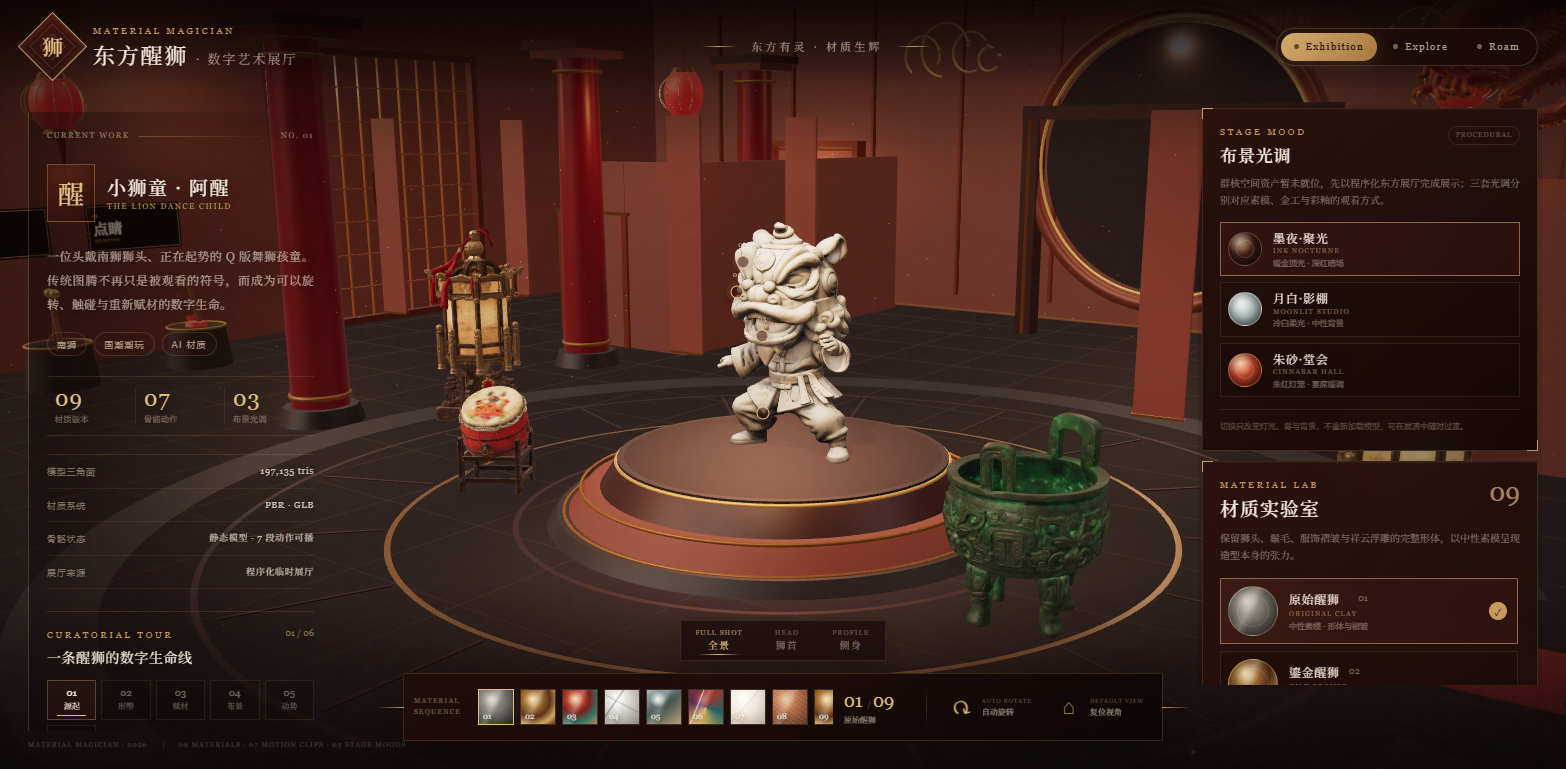
\includegraphics[width=\linewidth]{01-exhibition}
\caption{首屏：展台观察模式下的素模与展厅。左侧为作品展签与策展导览，右侧为布景光调、材质实验室与技术视图，底部为材质序列与观察机位。}
\end{figure}

画面中可以看到三层信息同时存在：中央是角色本身，左前方是 Lux3D 生成的醒狮鼓，右前方是生成的铜香炉，背景是盘龙与宫灯。

\subsection{材质对比}
\begin{figure}[H]
\centering
\begin{subfigure}{0.32\linewidth}
  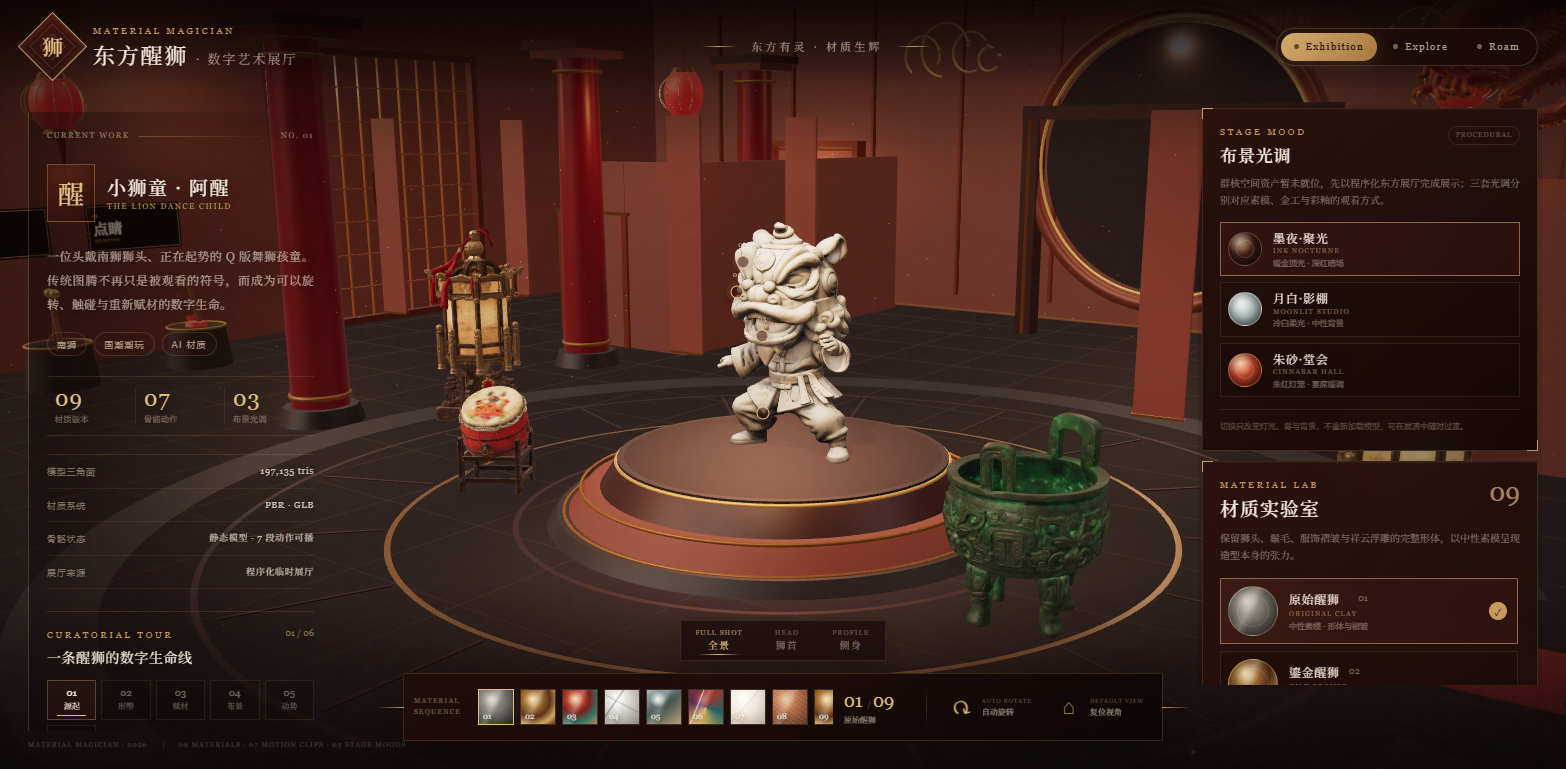
\includegraphics[width=\linewidth]{01-exhibition}
  \caption{素模}
\end{subfigure}\hfill
\begin{subfigure}{0.32\linewidth}
  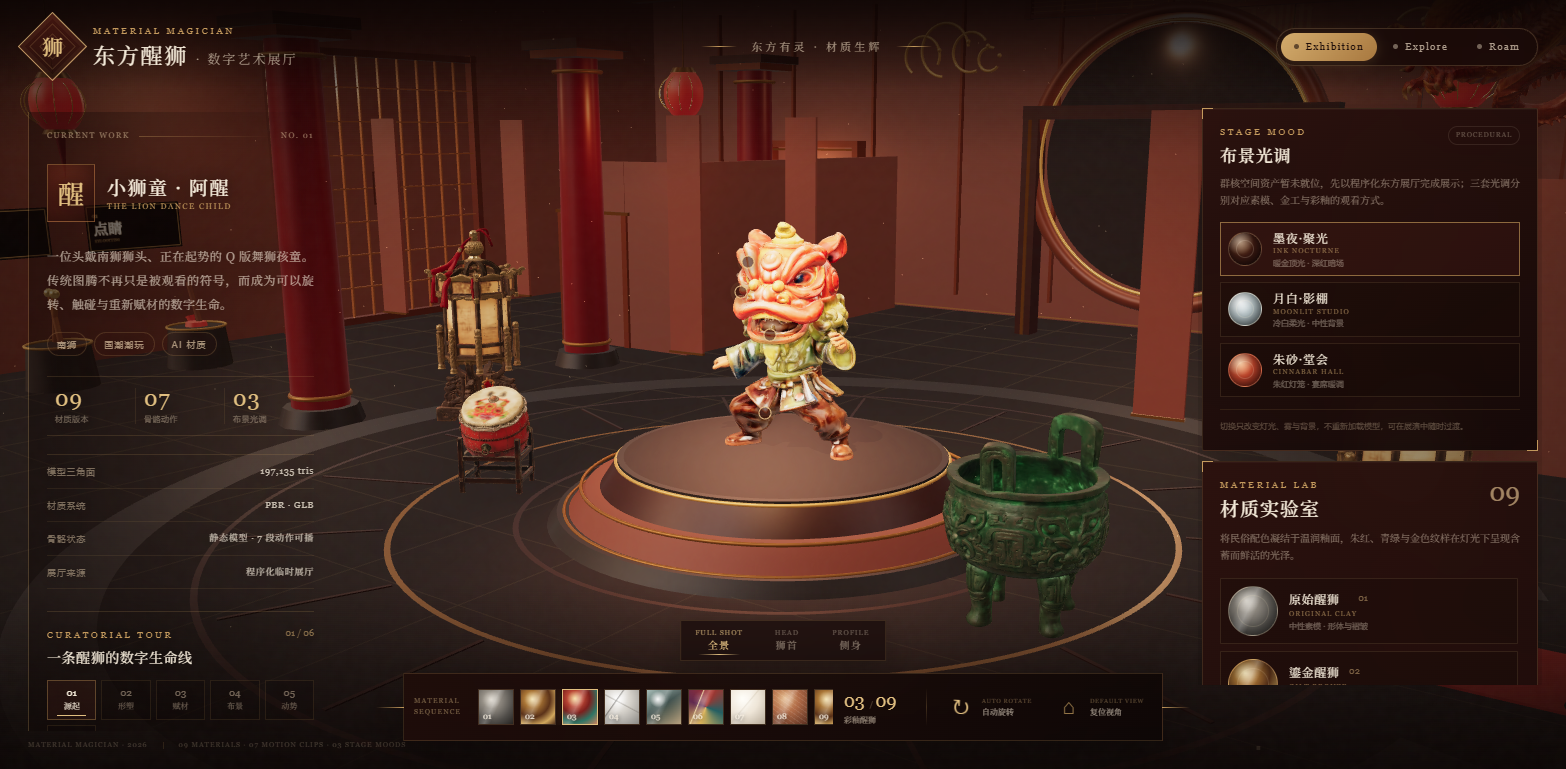
\includegraphics[width=\linewidth]{02-ceramic}
  \caption{彩釉}
\end{subfigure}\hfill
\begin{subfigure}{0.32\linewidth}
  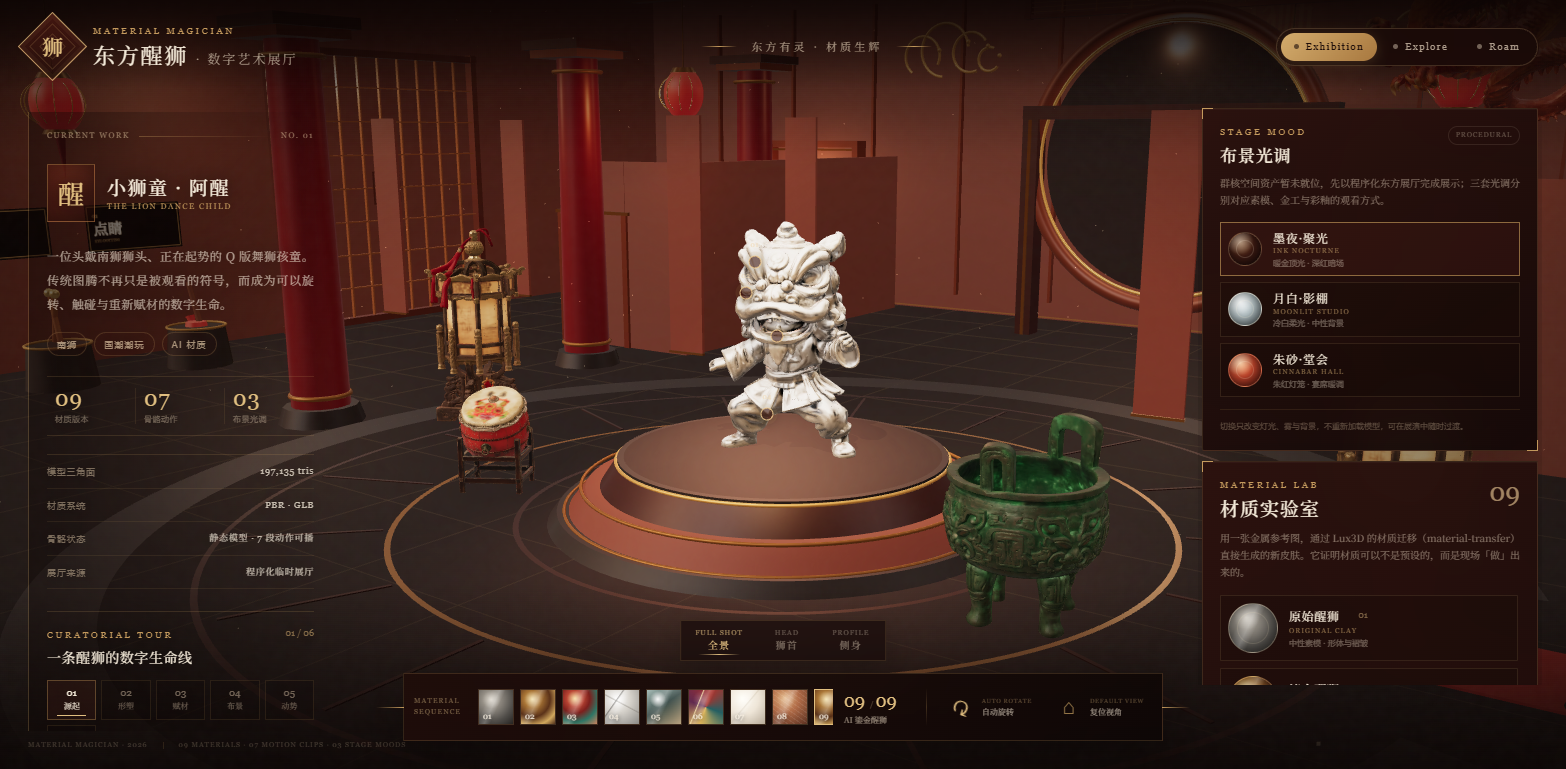
\includegraphics[width=\linewidth]{03-ai-metal}
  \caption{AI 鎏金}
\end{subfigure}
\caption{同一副几何的三套材质。左：中性素模，用于观察形体；中：八套预设材质之一的彩釉；右：由 Lux3D 材质迁移现场生成的「AI 鎏金」。}
\end{figure}

三张图使用同一机位、同一布景，只有材质不同，因此可以直接比较高光位置、粗糙度与颜色倾向的差异。右图的金属反射明显强于左图，这是材质迁移把参考图的金属度与粗糙度一并迁移过来的结果。

\subsection{角色漫游}
\begin{figure}[H]
\centering
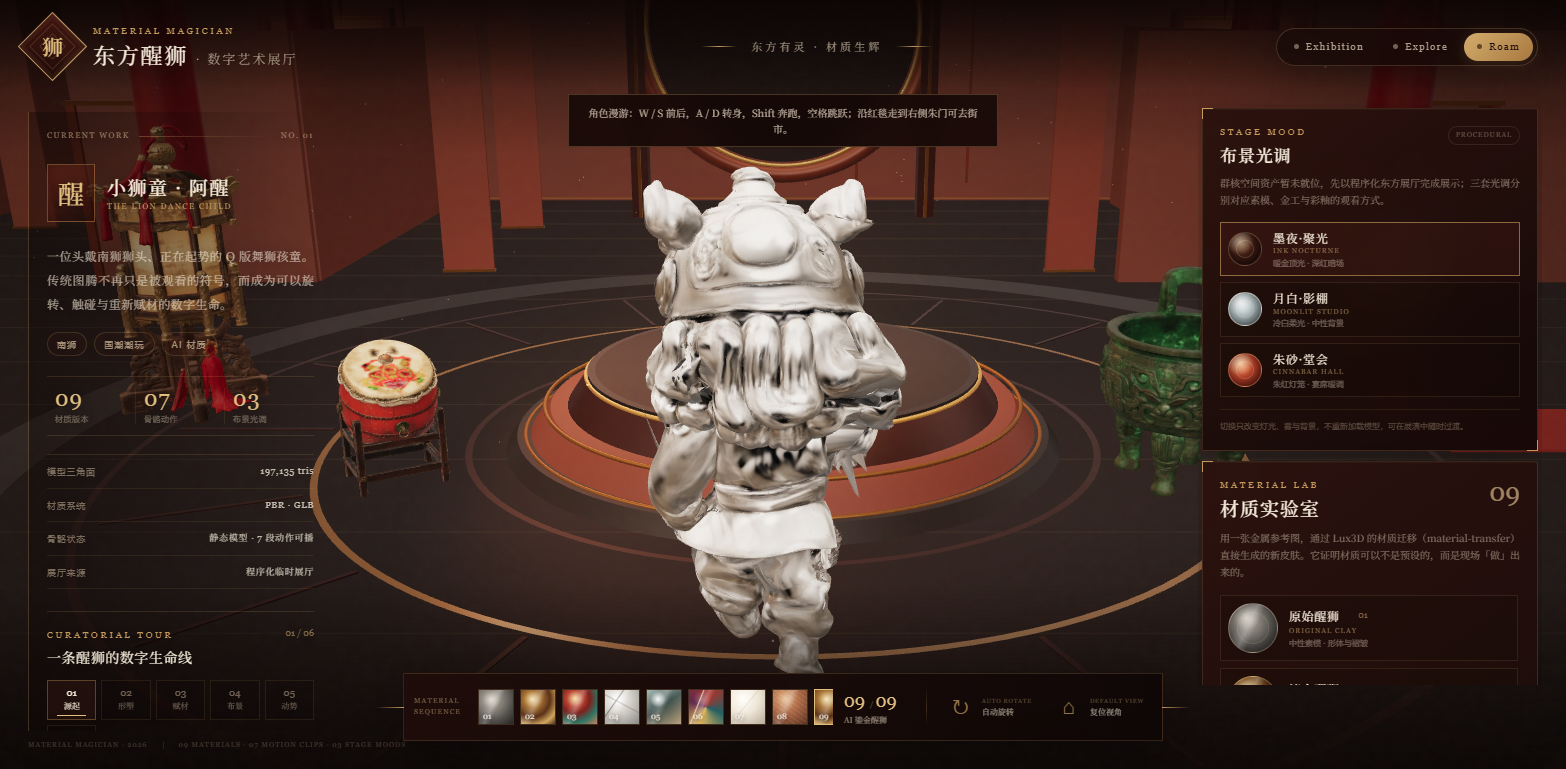
\includegraphics[width=0.86\linewidth]{06-roam}
\caption{Roam 模式：舞狮本人作为可操控角色，相机第三人称跟随。W/S 前后、A/D 转身、Shift 奔跑、空格跳跃。}
\end{figure}

进入漫游后，自动旋转暂停、部位热点与机位条隐藏，画面交给角色与空间本身。

\subsection{街市与全景}
\begin{figure}[H]
\centering
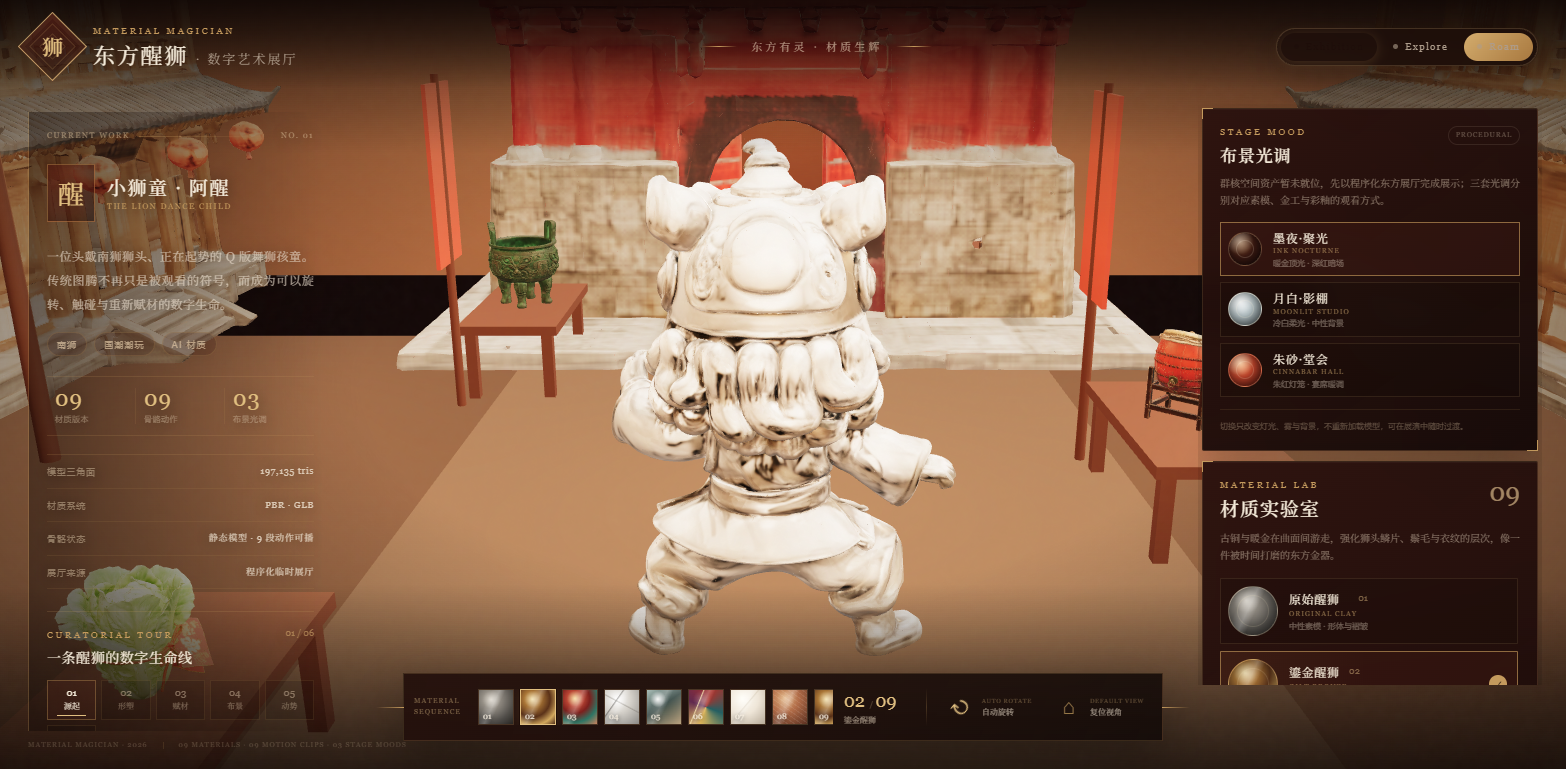
\includegraphics[width=\linewidth]{street}
\caption{长安街市：门楼、香炉、鼓与摊位，两侧为生成式酒楼，红光为场外补光。}
\end{figure}

街市与展厅共用同一渲染循环，因此额外补了方向光与半球光，否则 12 米外的立面会黑成一片。

\begin{figure}[H]
\centering
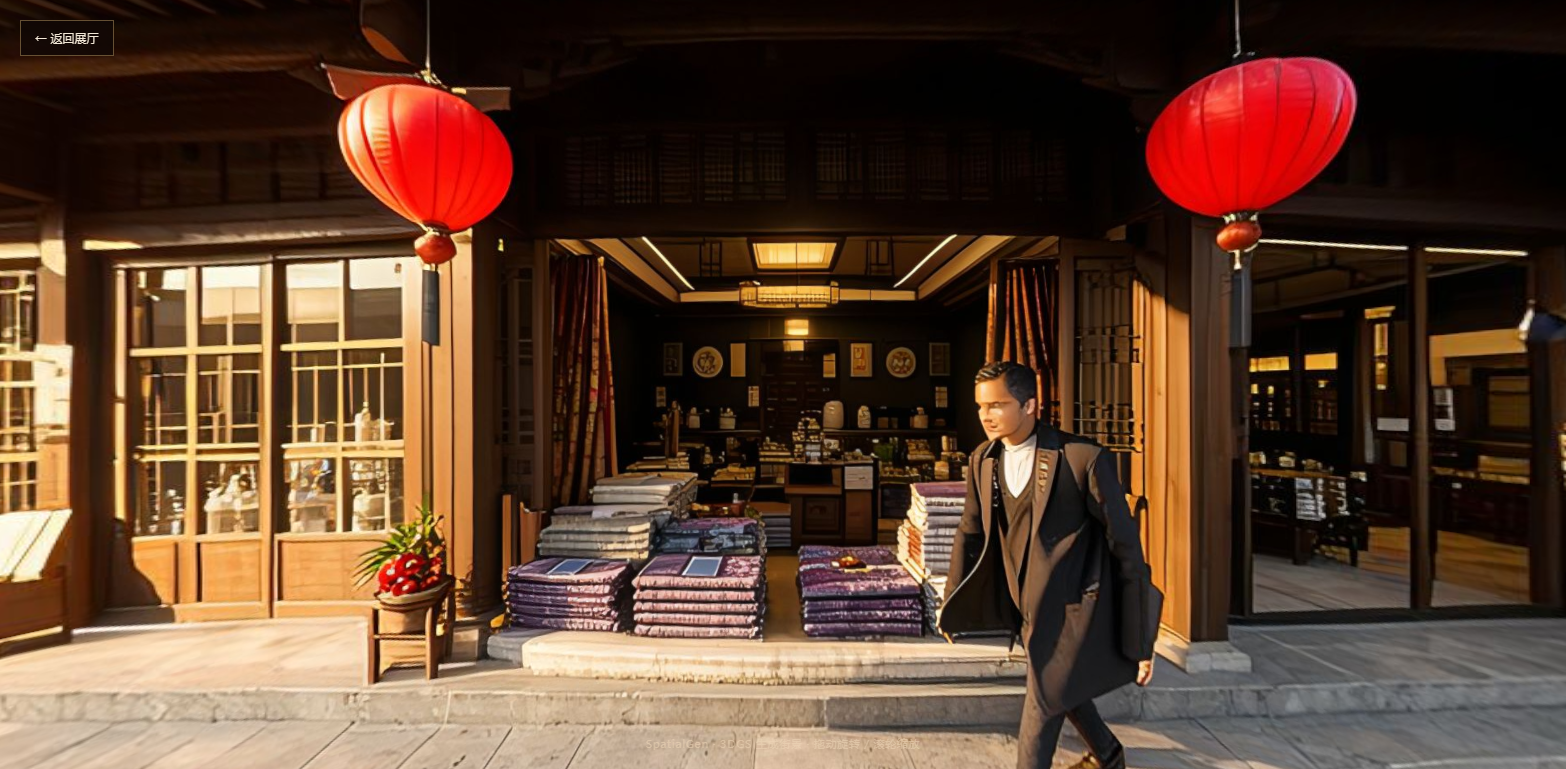
\includegraphics[width=\linewidth]{pano}
\caption{SpatialGen 全景街景：3DGS 的 spz 为 v3、库不支持，改用同一空间的等距柱状全景图，1.1MB、秒开。}
\end{figure}


% ============================================================
\section{与游戏引擎结合的可行性}

课程讨论中曾评估把项目迁移到 Unity 或 Blender 的可行性，结论如下。

\begin{table}[H]
\centering
\small
\caption{三条迁移路径}
\begin{tabular}{@{}p{2.6cm}p{4.2cm}p{3.2cm}p{4.0cm}@{}}
\toprule
路径 & 收益 & 成本 & 判断 \\
\midrule
Blender 做资产管线 & 合并动作、减面、LOD、烘焙 & 1--2 天 & 推荐 \\
Unity / Unreal 运行时 & 骨骼重定向、画质、离线打包 & 2--4 周重写 & 仅在必须离开浏览器时 \\
Blender 出片 + 现有 Web & 高质量渲染图与转台视频 & 3--5 天 & 低风险备选 \\
\bottomrule
\end{tabular}
\end{table}

关键判断：资产是 GLB，迁移本身不难；难的是**展厅是程序化代码而不是模型**，以及前端近千行的交互逻辑需要在 C\#/蓝图里重写。

% ============================================================
\section{未来工作}

\begin{enumerate}[itemsep=2pt]
  \item \textbf{资产合并}：用 Blender 把九段动作合并到一个带骨骼的主模型，体积可降约 70\%；
  \item \textbf{浏览器内材质共创}：增加本地代理，Key 留在服务端，实现「拖图即生成」；
  \item \textbf{多场景叙事}：再生成祠堂、练功房两个 3DGS 场景，用门串成三进空间；
  \item \textbf{空间理解}：用 \texttt{spatial-understanding} 为 3DGS 场景生成可行走区域与摆放点；
  \item \textbf{自动展演}：把「材质 $\times$ 光调 $\times$ 动作」编排为可一键播放的演示序列；
  \item \textbf{组合预设}：为「鎏金+直拳」「彩釉+跳舞」这类组合提供一键切换。
\end{enumerate}

% ============================================================
\section{结论}

项目把一尊静态 AI 素模扩展为可赋材、可动作、可讲述、可漫游的三维叙事空间，并把文生 3D、材质迁移、场景生成三类生成能力真正接入展陈流程。系统在浏览器内可稳定展示，核心难点集中在三处：动作与材质的解耦、根位移的处理、以及生成资产的接入与鉴权。当前版本的短板是资产体积与 3DGS 的交互能力，后续应优先解决资产合并与浏览器内共创。

% ============================================================
\appendix
\section{迭代索引}

\begin{longtable}{@{}clp{9.4cm}@{}}
\toprule
轮次 & 主题 & 关键改动 \\
\midrule
\endhead
01 & 展示界面 & 布景光调、三段材质、机位与快捷键 \\
02 & 动作扩容 & 新增 4 段动作，动作与材质解耦 \\
03 & 八套材质 & 材质全开、奔跑翻滚原地化 \\
04 & 内容加厚 & 材质档案、技术视图 \\
05 & 部位热点 & 五处热点与说明卡 \\
06 & 背景盘龙 & 龙模型接入与浮动 \\
07 & 醒狮鼓 & Lux3D 文生 3D 第一件 \\
08 & 铜香炉 & 大型摆件与通用加载器 \\
09 & 展厅放大 & 38$\times$42$\times$10、宫灯、点击展品 \\
10 & 提亮与屏风 & 洗墙光、盘龙巡游、壁龛、折屏 \\
11 & 侧室与漫游 & 门洞侧室、第三人称漫游 \\
12 & 街市与行人 & 开门、长安街、三个行人 \\
13 & 门与手感 & 红毯引导、阻尼移动、屏风减半 \\
14 & SpatialGen & 3DGS 街景生成与接入 \\
15 & 故事长廊 & 五章展台 \\
16 & 练功房 & 四件训练器械 \\
17 & 材质迁移 & 第 9 套材质与上传脚本 \\
18 & 动作分组 & 跳跃/滑铲三合一、蹲伏独立，Roam 新增 C/X \\
19 & 3DGS 优化 & 预取、加载层、超时回退 \\
20 & 按键提示 & 动作面板按键条、故事道具生成、过门修复 \\
21 & 传送门 & 侧栏传送、门楼阁楼、街市放大 \\
22 & 街市排楼 & 酒楼克隆成排、传送 teleport \\
23 & 四类建筑 & 酒楼/客栈/城门/店铺 \\
24 & 全景兜底 & spz v3 不兼容，改用 ply 与全景 \\
25 & 街市重做 & 两层店铺、补光、道具 \\
26 & 摊位道具 & 五处摊位与生成道具 \\
27 & 清理 & 移除长方体店铺，只留生成建筑 \\

\bottomrule
\end{longtable}

\section{生成任务记录}

\begin{table}[H]
\centering
\small
\caption{API 调用记录}
\begin{tabular}{@{}llll@{}}
\toprule
能力 & 任务 / 标识 & 耗时 & 产出 \\
\midrule
text-to-3d & 4564027 & 约 80s & 醒狮鼓 \\
text-to-3d & 4564131 & 约 70s & 铜香炉 \\
text-to-3d & 4564212 & 约 40s & 宫灯 \\
world/v1 & 3FO4K4RJ1HA6 & 约 16min & 长安街市 3DGS \\
material-transfer & 4580404 & 约 7min & AI 鎏金 \\
text-to-3d & 4587284 / 4587286 & 约 60s & 门楼 / 阁楼 \\
text-to-3d & 4589436 & 约 70s & 唐式酒楼 \\
text-to-3d & 4586827--4586838 & 约 60s ×5 & 故事展台道具 \\

\bottomrule
\end{tabular}
\end{table}

\section{运行与复现}

\begin{lstlisting}
npm install
npm run dev            # 本地开发
npm run build          # 生产构建
npm run material -- assets/references/青铜.png ai-bronze
\end{lstlisting}


\end{document}
